        %%******************************************%%
        %%                                          %%
        %%        Modello di tesi di laurea         %%
        %%            di Andrea Giraldin            %%
        %%                                          %%
        %%             2 novembre 2012              %%
        %%                                          %%
        %%******************************************%%


% I seguenti commenti speciali impostano:
% 1. 
% 2. PDFLaTeX come motore di composizione;
% 3. tesi.tex come documento principale;
% 4. il controllo ortografico italiano per l'editor.

% !TEX encoding = UTF-8
% !TEX TS-program = pdflatex
% !TEX root = tesi.tex
% !TEX spellcheck = it-IT

\documentclass[10pt,                    % corpo del font principale
               a4paper,                 % carta A4
               twoside,                 % impagina per fronte-retro
               openright,               % inizio capitoli a destra
               english,                 
               italian,                 
               ]{book}    

\usepackage[utf8]{inputenc}             % codifica di input; anche [latin1] va bene
                                        % NOTA BENE! va accordata con le preferenze dell'editor

%**************************************************************
% Importazione package
%************************************************************** 

% Mie personalizzazioni
\usepackage{float}											% float delle immagini

\usepackage{enumitem}										% enumerate con testo divisorio


%\usepackage{amsmath,amssymb,amsthm}    % matematica

\usepackage[english, italian]{babel}    % per scrivere in italiano e in inglese;
                                        % l'ultima lingua (l'italiano) risulta predefinita

\usepackage{bookmark}                   % segnalibri

\usepackage{caption}                    % didascalie

\usepackage{chngpage,calc}              % centra il frontespizio

\usepackage{csquotes}                   % gestisce automaticamente i caratteri (")

\usepackage{emptypage}                  % pagine vuote senza testatina e piede di pagina

\usepackage{epigraph}					% per epigrafi

\usepackage{eurosym}                    % simbolo dell'euro

\usepackage[T1]{fontenc}                % codifica dei font:
                                        % NOTA BENE! richiede una distribuzione *completa* di LaTeX

%\usepackage{indentfirst}               % rientra il primo paragrafo di ogni sezione

\usepackage{graphicx}                   % immagini

\usepackage{hyperref}                   % collegamenti ipertestuali



\usepackage[binding=5mm]{layaureo}      % margini ottimizzati per l'A4; rilegatura di 5 mm

\usepackage{listings}                   % codici

\usepackage{microtype}                  % microtipografia

\usepackage{mparhack,fixltx2e,relsize}  % finezze tipografiche

\usepackage{nameref}                    % visualizza nome dei riferimenti                                      

\usepackage[font=small]{quoting}        % citazioni

\usepackage{subfig}                     % sottofigure, sottotabelle

\usepackage[italian]{varioref}          % riferimenti completi della pagina

\usepackage[dvipsnames]{xcolor}         % colori

\usepackage{booktabs}                   % tabelle                                       
\usepackage{tabularx}                   % tabelle di larghezza prefissata                                    
\usepackage{longtable}                  % tabelle su più pagine                                        
\usepackage{ltxtable}                   % tabelle su più pagine e adattabili in larghezza

\usepackage[toc, acronym]{glossaries}   % glossario
                                        % per includerlo nel documento bisogna:
                                        % 1. compilare una prima volta tesi.tex;
                                        % 2. eseguire: makeindex -s tesi.ist -t tesi.glg -o tesi.gls tesi.glo
                                        % 3. eseguire: makeindex -s tesi.ist -t tesi.alg -o tesi.acr tesi.acn
                                        % 4. compilare due volte tesi.tex.

\usepackage[backend=biber,style=verbose-ibid,hyperref,backref]{biblatex}
                                        % eccellente pacchetto per la bibliografia; 
                                        % produce uno stile di citazione autore-anno; 
                                        % lo stile "numeric-comp" produce riferimenti numerici
                                        % per includerlo nel documento bisogna:
                                        % 1. compilare una prima volta tesi.tex;
                                        % 2. eseguire: biber tesi
                                        % 3. compilare ancora tesi.tex.

%**************************************************************
% file contenente le impostazioni della tesi
%**************************************************************

%**************************************************************
% Frontespizio
%**************************************************************
\newcommand{\myName}{Autore}                                    % autore
\newcommand{\myTitle}{Titolo della tesi}                    
\newcommand{\myDegree}{Tesi di laurea triennale}                % tipo di tesi
\newcommand{\myUni}{Università degli Studi di Padova}           % università
\newcommand{\myFaculty}{Corso di Laurea in Informatica}         % facoltà
\newcommand{\myDepartment}{Dipartimento di Matematica}          % dipartimento
\newcommand{\myProf}{Professore}                                % relatore
\newcommand{\myLocation}{Padova}                                % dove
\newcommand{\myAA}{2012-2013}                                   % anno accademico
\newcommand{\myTime}{Dec 2012}                                  % quando


%**************************************************************
% Impostazioni di impaginazione
% see: http://wwwcdf.pd.infn.it/AppuntiLinux/a2547.htm
%**************************************************************

\setlength{\parindent}{14pt}   % larghezza rientro della prima riga
\setlength{\parskip}{0pt}   % distanza tra i paragrafi


%**************************************************************
% Impostazioni di biblatex
%**************************************************************
\bibliography{bibliografia} % database di biblatex 

\defbibheading{bibliography}
{
    \cleardoublepage
    \phantomsection 
    \addcontentsline{toc}{chapter}{\bibname}
    \chapter*{\bibname\markboth{\bibname}{\bibname}}
}

\setlength\bibitemsep{1.5\itemsep} % spazio tra entry

\DeclareBibliographyCategory{opere}
\DeclareBibliographyCategory{web}

\addtocategory{opere}{womak:lean-thinking}
\addtocategory{web}{site:agile-manifesto}

\defbibheading{opere}{\section*{Riferimenti bibliografici}}
\defbibheading{web}{\section*{Siti Web consultati}}


%**************************************************************
% Impostazioni di caption
%**************************************************************
\captionsetup{
    tableposition=top,
    figureposition=bottom,
    font=small,
    format=hang,
    labelfont=bf
}

%**************************************************************
% Impostazioni di glossaries
%**************************************************************

%**************************************************************
% Acronimi
%**************************************************************
\renewcommand{\acronymname}{Acronimi e abbreviazioni}

\newacronym[description={\glslink{apig}{Application Program Interface}}]
    {api}{API}{Application Program Interface}
		
\newacronym[description={\glslink{cdng}{Content Delivery Network}}]
		{cdn}{CDN}{Content Delivery Network}

\newacronym[description={\glslink{crudg}{Create Read Update Delete}}]
	{crud}{CRUD}{Create Read Update Delete}
	
\newacronym[description={\glslink{cssg}{Cascading Style Sheet}}]
	{css}{CSS}{Cascading Style Sheet}
	
\newacronym[description={\glslink{e2eg}{End-To-End}}]
	{e2e}{E2E}{End-To-End}

\newacronym[description={\glslink{hateoasg}{Hypermedia as the Engine of Application State}}]
	{hateoas}{HATEOAS}{Hypermedia as the Engine of Application State}

\newacronym[description={\glslink{htmlg}{HyperText Markup Language}}]
	{html}{HTML}{HyperText Markup Language}
	
\newacronym[description={\glslink{httpg}{HyperText Transfer Protocol}}]
	{http}{HTTP}{HyperText Transfer Protocol}

\newacronym[description={\glslink{ictg}{Information and Communication Technology}}]
	{ict}{ICT}{Information and Communication Technology}

\newacronym[description={\glslink{ideg}{Integrated Development Environment}}]
	{ide}{IDE}{Integrated Development Environment}

\newacronym[description={\glslink{mvcg}{Model View Controller}}]
	{mvc}{MVC}{Model View Controller}

\newacronym[description={\glslink{npmg}{Node Package Manager}}]
	{npm}{NPM}{Node Package Manager}
		
\newacronym[description={\glslink{restg}{Representational State Transfer}}]
	{rest}{REST}{Representational State Transfer}
	
\newacronym[description={\glslink{soapg}{Simple Object Access Protocol}}]
  {soap}{SOAP}{Simple Object Access Protocol}
	
\newacronym[description={\glslink{spag}{Single Page Application}}]
	{spa}{SPA}{Single Page Application}

\newacronym[description={\glslink{umlg}{Unified Modeling Language}}]
    {uml}{UML}{Unified Modeling Language}

%**************************************************************
% Glossario
%**************************************************************
%\renewcommand{\glossaryname}{Glossario}

%\newglossaryentry{angularjs}
%{
%	name=\glslink{angularjs}{AngularJS}
%	sort=angularjs,
%	description={comunemente noto con il nome "Angular", è un framework open source mantenuto da %
%\emph{Google} e da una comunità di sviluppatori individuali e corporazioni. Il suo fine principale è la creazione di Single Page Application, semplificando la codifica e il testing. L'architettura di base di Angular è il pattern \emph{MVC}.}
%}

\newglossaryentry{apig}
{
    name=\glslink{api}{API},
    text=Application Program Interface,
    sort=api,
    description={in informatica con il termine \emph{Application Programming Interface API} (ing. interfaccia di programmazione di un'applicazione) si indica ogni insieme di procedure disponibili al programmatore, di solito raggruppate a formare un set di strumenti specifici per l'espletamento di un determinato compito all'interno di un certo programma. La finalità è ottenere un'astrazione, di solito tra l'hardware e il programmatore o tra software a basso e quello ad alto livello semplificando così il lavoro di programmazione.}
}

\newglossaryentry{backend}
{
	name=\glslink{backend}{Backend},
	sort=backend,
	description={un'applicazione o un programma backend serve indirettamente come supporto ai servizi del frontend, solitamente essendo vicino alla risorsa richiesta o avendo la capacità di comunicare con data risorsa. L'applicazione backend può interagire direttamente con il frontend oppure, forse più tipicamente, è un programma chiamato da un programma intermediario che si inserisce tra le attività del frontend e del backend.}
}

\newglossaryentry{cdng}
{
	name=\glslink{cdn}{CDN},
	text=Content Delivery Network,
	sort=cdn,
	description={sistema di computer collegati in rete attraverso Internet, che collaborano in maniera trasparente, sotto forma di sistema distribuito, per distribuire contenuti (specialmente contenuti multimediali di grandi dimensioni in termini di banda) agli utenti finali ed erogare servizi e file di generi diversi.}
}

\newglossaryentry{compliance}
{
	name=\glslink{compliance}{Compliance},
	sort=compliance,
	description={atto di essere in allineamento con linee guida, regolamentazioni e/o legislazioni.}
}

\newglossaryentry{crudg}
{
	name=\glslink{crud}{CRUD},
	text=Create Read Update Delete,
	sort=crud,
	description={con la sigla \emph{CRUD} si rappresenta l'insieme delle quattro operazioni basilari su dei dati persistenti, ovvero creazione, lettura, modifica ed eliminazione.}
}

\newglossaryentry{cssg}
{
	name=\glslink{css}{CSS},
	text=Cascading Style Sheet,
	sort=css,
	description={linguaggio usato per definire la formattazione di documenti HTML, XHTML e XML e relative pagine web. Le regole per comporre il CSS sono contenute in un insieme di direttive (Recommendations) emanate a partire dal 1996 dal W3C.\\
L'introduzione del CSS si è resa necessaria per separare i contenuti dalla formattazione e permettere una programmazione più chiara e facile da utilizzare, sia per gli autori delle pagine HTML che per gli utenti, garantendo contemporaneamente anche il riuso di codice ed una sua più facile manutenibilità.}
}

\newglossaryentry{e2eg}
{
	name=\glslink{e2e}{E2E},
	text=End-To-End,
	sort=ete,
	description={acronimo di \emph{End-To-End}, rappresenta quella categoria di test che si prefigge l'obiettivo di testare il comportamento di un utente su un sistema, usualmente automatizzando gli input utente previsti ed esaminando che i risultati attesi siano rispettati.}
}

\newglossaryentry{frontend}
{
	name=\glslink{frontend}{Frontend},
	sort=frontend,
	description={nel campo della progettazione software il front end è la parte di un sistema software che gestisce l'interazione con l'utente o con sistemi esterni che producono dati di ingresso (es. interfaccia utente con un form).}
}

\newglossaryentry{governance}
{
	name=\glslink{governance}{Governance},
	sort=governance,
	description={L'IT Governance è responsabilità diretta del consiglio di amministrazione e del management esecutivo. \`{E} parte integrante della governance aziendale ed è costituita dalla direzione, dalla struttura organizzativa e dai processi in grado di assicurare che l'IT sostenga ed estenda gli obiettivi e le strategie dell'organizzazione.}
}

\newglossaryentry{hateoasg}
{
	name=\glslink{hateoas}{HATEOAS},
	text=HATEOAS,
	sort=hateoas,
	description={vincolo delle applicazioni basate su architettura REST che le distingue dalla maggior parte delle altre applicazioni web. Il principio consiste in un client che interagisce con un'applicazione web esclusivamente attraverso gli ipermedia forniti dinamicamente dai server dell'applicazione stessa. Un client REST non necessita così di nessuna conoscenza a priori per interagire con una particolare applicazione o server che vada oltre la normale comprensione degli ipermedia.}
}

\newglossaryentry{htmlg}
{
	name=\glslink{html}{HTML},
	text=HTML,
	sort=html,
	description={linguaggio di markup solitamente usato per la formattazione e impaginazione di documenti ipertestuali disponibili nel World Wide Web sotto forma di pagine web.}
}

\newglossaryentry{httpg}
{
	name=\glslink{http}{HTTP},
	text=HTTP,
	sort=http,
	description={tradotto in \emph{protocollo di trasferimento di un ipertesto}, è usato come principale protocollo per la trasmissione d'informazioni sul web.}
}

\newglossaryentry{ictg}
{
	name=\glslink{ict}{ICT},
	text=ICT,
	sort=ict,
	description={acronimo di \emph{Information and Communication Technology}, tradotto in Tecnologie dell’informazione e della comunicazione. Sono l'insieme dei metodi e delle tecnologie che realizzano i sistemi di trasmissione, ricezione ed elaborazione di informazioni.}
}

\newglossaryentry{ideg}
{
	name=\glslink{ide}{IDE}
	text=IDE,
	sort=ide,
	description={si traduce in italiano come Ambiente di Sviluppo Integrato. Un IDE è un software che, in fase di programmazione, aiuta i programmatori nello sviluppo del codice sorgente di un programma. Spesso l'IDE aiuta lo sviluppatore segnalando errori di sintassi del codice direttamente in fase di scrittura, oltre a tutta una serie di strumenti e funzionalità di supporto alla fase di sviluppo e debugging.}
}

\newglossaryentry{mvcg}
{
	name=\glslink{mvc}{MVC},
	text=MVC,
	sort=mvc,
	description={pattern architetturale software utilizzato nell'implementazione di interfacce utente. Divide l'applicazione software in tre parti interconnesse, così da separare la rappresentazione interna delle informazioni dal modo in cui tali informazioni sono presentate all'utente.}
}

\newglossaryentry{npmg}
{
	name=\glslink{npm}{NPM},
	text=NPM,
	sort=npm,
	description={package manager di JavaScript, usato di default da Node.js. Una volta installato Node.js, è possibile utilizzare anche NPM, dato che viene distribuito assieme a suddetto framework. Al suo interno si trovano tutti i maggiori framework ed utilities che si basano sul linguaggio JavaScript.}
}

\newglossaryentry{repository}
{
	name=\glslink{repository}{Repository},
	sort=repository,
	description={struttura di supporto su cui un software può essere progettato e realizzato. Alla base di un framework sono sempre presenti delle librerie di codice utilizzabili con uno o più linguaggi di programmazione; esse sono spesso corredate da una serie di strumenti di supporto allo sviluppo software, o altri strumenti ideati per aumentare la velocità di sviluppo del prodotto finito. Lo scopo di un framework è quello di far risparmiare allo sviluppatore la riscrittura di codice già scritto precedentemente per fini simili.}
}

\newglossaryentry{restg}
{
	name=\glslink{rest}{REST},
	text=REST,
	sort=rest,
	description={REST si riferisce ad un insieme di principi di architetture di rete, i quali delineano come le risorse sono definite e indirizzate. Il termine è spesso usato nel senso di descrivere ogni semplice interfaccia che trasmette dati su HTTP senza un livello opzionale.}
}

\newglossaryentry{soapg}
{
  name=\glslink{soap}{SOAP},
	text=SOAP,
	sort=soap,
	description={acronimo di \emph{Simple Object Access Protocol}, è un protocollo leggero per lo scambio di messaggi tra componenti software, tipicamente nella forma di componentistica software. La parola object manifesta che l'uso del protocollo dovrebbe effettuarsi secondo il paradigma della programmazione orientata agli oggetti.}
}

\newglossaryentry{spag}
{
	name=\glslink{spa}{SPA},
	text=SPA,
	sort=spa,
	description={una Single Page (Web) Application è un'applicazione web o semplicemente un sito che si propone di realizzare un comportamento più espressivo rispetto ad un'applicazione desktop. In una \emph{SPA}, il codice necessario viene caricato al caricamento della pagina e tutti i contenuti vengono visualizzati dinamicamente, mentre tutte le comunicazioni con il server vengono nascoste all'utente.}
}

\newglossaryentry{spring}
{
	name=\glslink{spring}{Spring},
	sort=spring,
	description={framework open source per lo sviluppo di applicazioni su piattaforma Java. Spring fornisce un modello comprensivo di programmazione e configurazione per applicazioni \emph{enterprise} basate sulla piattaforma Java.}
}

\newglossaryentry{stub}
{
	name=\glslink{stub}{Stub},
	sort=stub,
	description={porzione di codice utilizzata in sostituzione di altre funzionalità software. Uno stub può simulare il comportamento di codice esistente e temporaneo sostituto di codice ancora da sviluppare. Gli stub sono perciò molto utili durante il porting di software, l'elaborazione distribuita e in generale durante lo sviluppo di software e il software testing.}
}
		
\newglossaryentry{umlg}
{
    name=\glslink{uml}{UML},
    text=UML,
    sort=uml,
    description={in ingegneria del software \emph{UML, Unified Modeling Language} (ing. linguaggio di modellazione unificato) è un linguaggio di modellazione e specifica basato sul paradigma object-oriented. L'\emph{UML} svolge un'importantissima funzione di ``lingua franca'' nella comunità della progettazione e programmazione a oggetti. Gran parte della letteratura di settore usa tale linguaggio per descrivere soluzioni analitiche e progettuali in modo sintetico e comprensibile a un vasto pubblico}
}
 % database di termini
\makeglossaries


%**************************************************************
% Impostazioni di graphicx
%**************************************************************
\graphicspath{{immagini/}} % cartella dove sono riposte le immagini


%**************************************************************
% Impostazioni di hyperref
%**************************************************************
\hypersetup{
    %hyperfootnotes=false,
    %pdfpagelabels,
    %draft,	% = elimina tutti i link (utile per stampe in bianco e nero)
    colorlinks=true,
    linktocpage=true,
    pdfstartpage=1,
    pdfstartview=FitV,
    % decommenta la riga seguente per avere link in nero (per esempio per la stampa in bianco e nero)
    %colorlinks=false, linktocpage=false, pdfborder={0 0 0}, pdfstartpage=1, pdfstartview=FitV,
    breaklinks=true,
    pdfpagemode=UseNone,
    pageanchor=true,
    pdfpagemode=UseOutlines,
    plainpages=false,
    bookmarksnumbered,
    bookmarksopen=true,
    bookmarksopenlevel=1,
    hypertexnames=true,
    pdfhighlight=/O,
    %nesting=true,
    %frenchlinks,
    urlcolor=webbrown,
    linkcolor=RoyalBlue,
    citecolor=webgreen,
    %pagecolor=RoyalBlue,
    %urlcolor=Black, linkcolor=Black, citecolor=Black, %pagecolor=Black,
    pdftitle={\myTitle},
    pdfauthor={\textcopyright\ \myName, \myUni, \myFaculty},
    pdfsubject={},
    pdfkeywords={},
    pdfcreator={pdfLaTeX},
    pdfproducer={LaTeX}
}

%**************************************************************
% Impostazioni di itemize
%**************************************************************
\renewcommand{\labelitemi}{$\ast$}

%\renewcommand{\labelitemi}{$\bullet$}
%\renewcommand{\labelitemii}{$\cdot$}
%\renewcommand{\labelitemiii}{$\diamond$}
%\renewcommand{\labelitemiv}{$\ast$}


%**************************************************************
% Impostazioni di listings
%**************************************************************
\lstset{
    language=[LaTeX]Tex,%C++,
    keywordstyle=\color{RoyalBlue}, %\bfseries,
    basicstyle=\small\ttfamily,
    %identifierstyle=\color{NavyBlue},
    commentstyle=\color{Green}\ttfamily,
    stringstyle=\rmfamily,
    numbers=none, %left,%
    numberstyle=\scriptsize, %\tiny
    stepnumber=5,
    numbersep=8pt,
    showstringspaces=false,
    breaklines=true,
    frameround=ftff,
    frame=single
} 


%**************************************************************
% Impostazioni di xcolor
%**************************************************************
\definecolor{webgreen}{rgb}{0,.5,0}
\definecolor{webbrown}{rgb}{.6,0,0}


%**************************************************************
% Altro
%**************************************************************

\newcommand{\omissis}{[\dots\negthinspace]} % produce [...]

% eccezioni all'algoritmo di sillabazione
\hyphenation
{
    ma-cro-istru-zio-ne
    gi-ral-din
}

\newcommand{\sectionname}{sezione}
\addto\captionsitalian{\renewcommand{\figurename}{figura}
                       \renewcommand{\tablename}{tabella}}

\newcommand{\glsfirstoccur}{\ap{{[g]}}}

\newcommand{\intro}[1]{\emph{\textsf{#1}}}

%**************************************************************
% Environment per ``rischi''
%**************************************************************
\newcounter{riskcounter}                % define a counter
\setcounter{riskcounter}{0}             % set the counter to some initial value

%%%% Parameters
% #1: Title
\newenvironment{risk}[1]{
    \refstepcounter{riskcounter}        % increment counter
    \par \noindent                      % start new paragraph
    \textbf{\arabic{riskcounter}. #1}   % display the title before the 
                                        % content of the environment is displayed 
}{
    \par\medskip
}

\newcommand{\riskname}{Rischio}

\newcommand{\riskdescription}[1]{\textbf{\\Descrizione:} #1.}

\newcommand{\risksolution}[1]{\textbf{\\Soluzione:} #1.}

%**************************************************************
% Environment per ``use case''
%**************************************************************
\newcounter{usecasecounter}             % define a counter
\setcounter{usecasecounter}{0}          % set the counter to some initial value

%%%% Parameters
% #1: ID
% #2: Nome
\newenvironment{usecase}[2]{
    \renewcommand{\theusecasecounter}{\usecasename #1}  % this is where the display of 
                                                        % the counter is overwritten/modified
    \refstepcounter{usecasecounter}             % increment counter
    \vspace{10pt}
    \par \noindent                              % start new paragraph
    {\large \textbf{\usecasename #1: #2}}       % display the title before the 
                                                % content of the environment is displayed 
    \medskip
}{
    \medskip
}

\newcommand{\usecasename}{UC}

\newcommand{\usecaseactors}[1]{\textbf{\\Attori Principali:} #1. \vspace{4pt}}
\newcommand{\usecasepre}[1]{\textbf{\\Precondizioni:} #1. \vspace{4pt}}
\newcommand{\usecasedesc}[1]{\textbf{\\Descrizione:} #1. \vspace{4pt}}
\newcommand{\usecasepost}[1]{\textbf{\\Postcondizioni:} #1. \vspace{4pt}}
\newcommand{\usecasealt}[1]{\textbf{\\Scenario Alternativo:} #1. \vspace{4pt}}

%**************************************************************
% Environment per ``namespace description''
%**************************************************************

\newenvironment{namespacedesc}{
    \vspace{10pt}
    \par \noindent                              % start new paragraph
    \begin{description} 
}{
    \end{description}
    \medskip
}

\newcommand{\classdesc}[2]{\item[\textbf{#1:}] #2}                     % file con le impostazioni personali

\begin{document}
%**************************************************************
% Materiale iniziale
%**************************************************************
\frontmatter
% !TEX encoding = UTF-8
% !TEX TS-program = pdflatex
% !TEX root = ../tesi.tex
% !TEX spellcheck = it-IT

%**************************************************************
% Frontespizio 
%**************************************************************
\begin{titlepage}

\begin{center}

\begin{LARGE}
\textbf{\myUni}\\
\end{LARGE}

\vspace{10pt}

\begin{Large}
\textsc{\myDepartment}\\
\end{Large}

\vspace{10pt}

\begin{large}
\textsc{\myFaculty}\\
\end{large}

\vspace{30pt}
\begin{figure}[htbp]
\begin{center}

\includegraphics[height=6cm]{logo-unipd}
\end{center}
\end{figure}
\vspace{30pt} 

\begin{LARGE}
\begin{center}
\textbf{\myTitle}\\
\end{center}
\end{LARGE}

\vspace{10pt} 

\begin{large}
\textsl{\myDegree}\\
\end{large}

\vspace{40pt} 

\begin{large}
\begin{flushleft}
\textit{Relatore}\\ 
\vspace{5pt} 
Prof. \myProf
\end{flushleft}

\vspace{0pt} 

\begin{flushright}
\textit{Laureando}\\ 
\vspace{5pt} 
\myName
\end{flushright}
\end{large}

\vspace{40pt}

\line(1, 0){338} \\
\begin{normalsize}
\textsc{Anno Accademico \myAA}
\end{normalsize}

\end{center}
\end{titlepage} 
% !TEX encoding = UTF-8
% !TEX TS-program = pdflatex
% !TEX root = ../tesi.tex
% !TEX spellcheck = it-IT

%**************************************************************
% Colophon
%**************************************************************
\clearpage
\phantomsection
\thispagestyle{empty}

\hfill

\vfill

\noindent\myName: \textit{\myTitle,}
\myDegree,
\textcopyright\ \myTime.
% !TEX encoding = UTF-8
% !TEX TS-program = pdflatex
% !TEX root = ../tesi.tex
% !TEX spellcheck = it-IT

%**************************************************************
% Dedica
%**************************************************************
\cleardoublepage
\phantomsection
\thispagestyle{empty}
\pdfbookmark{Dedica}{Dedica}

\vspace*{3cm}

\begin{center}
Lorem ipsum dolor sit amet, consectetuer adipiscing elit. \\ \medskip
--- Oscar Wilde    
\end{center}

\medskip

\begin{center}
Dedicato a ...
\end{center}

% !TEX encoding = UTF-8
% !TEX TS-program = pdflatex
% !TEX root = ../tesi.tex
% !TEX spellcheck = it-IT

%**************************************************************
% Sommario
%**************************************************************
\cleardoublepage
\phantomsection
\pdfbookmark{Sommario}{Sommario}
\begingroup
\let\clearpage\relax
\let\cleardoublepage\relax
\let\cleardoublepage\relax

\chapter*{Sommario}

Il presente documento descrive il lavoro svolto durante il periodo di Stage, della durata di circa trecento ore, dal laureando Mattia Sorgato presso l'azienda IKS s.r.l. Gli obbiettivi da raggiungere erano molteplici.\\
In primo luogo, l'ideazione e l'implementazione del \gls{front-end} di un software per la gestione del personale e dei progetti aziendali, per la quale scrittura è stato richiesto l'impiego del \emph{framework} AngularJS.\\
In secondo luogo, la scrittura delle \gls{api} necessarie alla stesura del \gls{back-end}.\\
Per garantire la qualità del codice, durante l'intero progetto l'approccio utilizzato è stato Test Driven.

%\vfill
%
%\selectlanguage{english}
%\pdfbookmark{Abstract}{Abstract}
%\chapter*{Abstract}
%
%\selectlanguage{italian}

\endgroup			

\vfill


% !TEX encoding = UTF-8
% !TEX TS-program = pdflatex
% !TEX root = ../tesi.tex
% !TEX spellcheck = it-IT

%**************************************************************
% Ringraziamenti
%**************************************************************
\cleardoublepage
\phantomsection
\pdfbookmark{Ringraziamenti}{ringraziamenti}

%\begin{flushright}{
%	\slshape    
%	``Life is really simple, but we insist on making it complicated''} \\ 
%	\medskip
%    --- Confucius
%\end{flushright}


\bigskip

\begingroup
\let\clearpage\relax
\let\cleardoublepage\relax
\let\cleardoublepage\relax

\chapter*{Ringraziamenti}

\noindent \textit{Innanzitutto, vorrei esprimere la mia gratitudine al Prof. Mauro Conti, relatore della mia tesi, per l'aiuto e il sostegno fornitomi durante la stesura del lavoro.}\\

\noindent \textit{Desidero ringraziare con affetto i miei genitori per il sostegno, il grande aiuto e per essermi stati vicini in ogni momento durante gli anni di studio.}\\

\noindent \textit{Ho desiderio di ringraziare poi i miei amici per tutti i bellissimi anni passati insieme e le mille avventure vissute.}\\
\bigskip

\noindent\textit{\myLocation, \myTime}
\hfill \myName

\endgroup


% !TEX encoding = UTF-8
% !TEX TS-program = pdflatex
% !TEX root = ../tesi.tex
% !TEX spellcheck = it-IT

%**************************************************************
% Indici
%**************************************************************
\cleardoublepage
\pdfbookmark{\contentsname}{tableofcontents}
\setcounter{tocdepth}{2}
\tableofcontents
%\markboth{\contentsname}{\contentsname} 
\clearpage

\begingroup 
    \let\clearpage\relax
    \let\cleardoublepage\relax
    \let\cleardoublepage\relax
    %*******************************************************
    % Elenco delle figure
    %*******************************************************    
    \phantomsection
    \pdfbookmark{\listfigurename}{lof}
    \listoffigures

    \vspace*{8ex}

    %*******************************************************
    % Elenco delle tabelle
    %*******************************************************
    \phantomsection
    \pdfbookmark{\listtablename}{lot}
    \listoftables
        
    \vspace*{8ex}
\endgroup

\cleardoublepage

\cleardoublepage

%**************************************************************
% Materiale principale
%**************************************************************
\mainmatter
% !TEX encoding = UTF-8
% !TEX TS-program = pdflatex
% !TEX root = ../tesi.tex
% !TEX spellcheck = it-IT

%**************************************************************
\chapter{Introduzione}
\label{cap:introduzione}
%**************************************************************

Introduzione al contesto applicativo.\\

\noindent Esempio di utilizzo di un termine nel glossario \\
\gls{api}. \\

\noindent Esempio di citazione in linea \\
\cite{site:agile-manifesto}. \\

\noindent Esempio di citazione nel pie' di pagina \\
citazione\footcite{womak:lean-thinking} \\

%**************************************************************
\section{L'azienda}

Descrizione dell'azienda.

%**************************************************************
\section{L'idea}

Il progetto \myTitle{} nasce come strumento di gestione interna delle competenze e dei progetti presenti in azienda. L'obiettivo di tale progetto è una migliore organizzazione del personale dedicato ai vari progetti, con una conseguente maggiore efficienza ed efficacia nell'assegnazione dei ruoli nei processi ed attività. Fino ad ora, all'interno di IKS, tale compito veniva svolto dalla consultazione e modifica di un foglio elettronico \emph{Excel}. Questa soluzione, oltre ad essere poco pratica e difficilmente manutenibile, ha portato all'esigenza di uno strumento più specifico ed espandibile. Da qui la nascita del progetto \myTitle{}.\\
L'applicazione sarà composta da un \gls{frontend} realizzato in \emph{AngularJS}, un \gls{backend} realizzato tramite \emph{Spring} e un database di persistenza. L'attività di Stage ha riguardato la realizzazione del frontend e la definizione delle \gls{api} \gls{rest} del backend. 
%definisci SPRING

Il personale aziendale inserisce le proprie competenze nel sistema, selezionate a partire da un elenco precompilato. 
Chi ha compiti di gestione utilizza lo strumento per vedere quali risorse può utilizzare per un
progetto. Ogni utente potrà inoltre tenere traccia dei vari progetti a cui ha collaborato, delle competenze acquisite e dei vari attestati ottenuti durante la carriera aziendale e non.
Si prefissa quindi come obiettivo la creazione di un portale aziendale unificato per una migliore gestione del personale ed il suo dislocamento all’interno dei progetti aziendali, oltre che alla gestione dei curricula vitae del personale aziendale.


%**************************************************************
\section{Organizzazione del testo}

\begin{description}
    \item[{\hyperref[cap:processi-metodologie]{Il secondo capitolo}}] descrive ...
    
    \item[{\hyperref[cap:descrizione-stage]{Il terzo capitolo}}] approfondisce ...
    
    \item[{\hyperref[cap:analisi-requisiti]{Il quarto capitolo}}] approfondisce ...
    
    \item[{\hyperref[cap:progettazione-codifica]{Il quinto capitolo}}] approfondisce ...
    
    \item[{\hyperref[cap:verifica-validazione]{Il sesto capitolo}}] approfondisce ...
    
    \item[{\hyperref[cap:conclusioni]{Nel settimo capitolo}}] descrive ...
\end{description}

Riguardo la stesura del testo, relativamente al documento sono state adottate le seguenti convenzioni tipografiche:
\begin{itemize}
	\item gli acronimi, le abbreviazioni e i termini ambigui o di uso non comune menzionati vengono definiti nel glossario, situato alla fine del presente documento;
	\item per la prima occorrenza dei termini riportati nel glossario viene utilizzata la seguente nomenclatura: \emph{parola}\glsfirstoccur;
	\item i termini in lingua straniera o facenti parti del gergo tecnico sono evidenziati con il carattere \emph{corsivo}.
\end{itemize}             % Introduzione
% !TEX encoding = UTF-8
% !TEX TS-program = pdflatex
% !TEX root = ../tesi.tex
% !TEX spellcheck = it-IT

%**************************************************************
\chapter{Processi e metodologie}
\label{cap:processi-metodologie}
%**************************************************************

\intro{Brevissima introduzione al capitolo}\\

%**************************************************************
\section{Processo sviluppo prodotto}

\subsection{Agile}
Agile è una metodologia di sviluppo nata in contrapposizione ad altri modelli più stringenti e formali, quali ad esempio il modello a Cascata o a Spirale.\\
I principi generali dell’Agile Programming sono descritti nell’Agile Manifesto\footcite{site:agile-manifesto}, e possono essere riassunti in quattro punti cardine:
\begin{itemize}
	\item \emph{individui e interazioni:} organizzazione e motivazione autonoma sono importanti, come lo sono le interazioni personali come la condivisione dello stesso luogo di sviluppo;
	\item \emph{software funzionante:} un prodotto che funziona è più utile e meglio accettato di documenti cartacei presentati agli acquirenti durante i meeting;
	\item \emph{collaborazione con gli acquirenti:} i requisiti non possono essere pienamente individuati all’inizio del ciclo di sviluppo del software. Perciò l’interazione con i clienti e gli stakeholder è estremamente importante;
	\item \emph{responsività al cambiamento:} i metodi agile sono focalizzati sul fornire risposte veloci al cambiamento e allo sviluppo continuo.
\end{itemize}
Lo sviluppo Agile permette di valutare ed eventualmente correggere la direzione durante il processo stesso. Questo risultato è ottenuto attraverso brevi e regolari iterazioni di lavoro, alla fine delle quali ogni team deve presentare un incremento del prodotto, considerandolo come una nuova feature applicabile e funzionante. Concentrandosi sulla ripetizione di cicli di lavoro brevi e definiti, proporzionati alla funzionalità da consegnare, le metodologie Agile si definiscono “iterative” o “incrementali”. Nel modello a cascata, i team di sviluppo hanno una sola opportunità di realizzare un aspetto del progetto nel modo giusto. Nel paradigma Agile, ogni aspetto dello sviluppo - requisiti, progettazione, ecc. - è continuamente rivisitato. Quando un team si ferma e rivaluta la direzione di un progetto ogni due settimane, è possibile cambiare tale direzione con facilità.\\
Questo approccio “ispeziona-e-adatta” riduce i costi e il tempo di consegna dello sviluppo. Dato che i vari team possono sviluppare software nello stesso tempo in cui individuano i requisiti, la “paralisi dell’analisi” ha meno probabilità di bloccare i progressi di un team. E siccome il ciclo di lavoro di un team è limitato a due settimane, gli stakeholder hanno opportunità ricorrenti di analizzare i rilasci del software e il loro feedback dal mercato.\\
La metodologia Agile si basa sul concetto di \emph{User Story}, ovvero un compito significativo che l'utente vuole poter svolgere attraverso il software realizzato. Le User Stories catturano il 'chi', 'cosa' e 'perché' di un requisito in maniera semplice e concisa.

\subsubsection{Kanban}
%storia
Kanban è un framework usato per implementare la metodologia agile. Negli anni ‘40, Toyota ottimizzò i suoi processi modellandoli come se fossero degli scaffali in un supermercato. I supermercati offrono una quantità di prodotti atti a soddisfare con il minimo spreco la domanda dei consumatori. Siccome i livelli di inventario sono conseguenti ai pattern di consumazione, il supermercato ottiene una significante efficienza ed ottimizzazione nella gestione dell’inventario.\\
Quando Toyota portò questa idea ai suoi piani di lavoro, i team (come ad esempio il team che aggiunge le portiere al telaio dell’auto) consegnavano una carta, o “kanban”, agli altri dipendenti (ad esempio, ai team che assemblano le portiere) per segnalare di aver ecceduto la capacità e di essere pronti a ritirare più materiale. Anche se la tecnologia di segnalazione si sia evoluta, questo sistema è ancora al centro della produzione “just in time”.\\
Kanban presenta lo stesso comportamento per i team software. Tramite la comparazione dell’ammontare del lavoro in progresso rispetto alla capacità del team, kanban fornisce agli stessi opzioni di pianificazione più flessibili, output più veloci, miglior concentrazione sui singoli compiti e trasparenza durante il ciclo di sviluppo.\\
%metodologia
Kanban è un metodo di gestione della consapevolezza del lavoro con un’enfasi particolare sulla consegna “just in time”, assicurandosi nel mentre che i membri del team non abbiano troppo lavoro rispetto alle loro capacità di carico. In questo approccio, il processo, dalla definizione dei task alla consegna al cliente, è mostrato visivamente ai partecipanti. I membri del team estraggono ogni unità di lavoro da una coda.
Kanban nel contesto dello sviluppo software può essere inteso come un sistema di gestione di processo visuale, che dice cosa produrre, quando e in quale quantità produrlo - ispirato dal sistema di produzione Toyota.\\
Nella sua forma più basilare, un sistema di kanban consiste di una grande lavagna appesa ad un muro con delle carte o dei postit organizzati in colonne con dei numeri su ogni colonna\footcite{site:kanban}.\\
Le carte rappresentano le unità di lavoro mentre attraversano il processo di sviluppo, rappresentato dalle colonne.\\
I limiti sono la differenza sostanziale tra una lavagna Kanban e un’altra storyboard qualsiasi. Limitando l’ammontare di Work-In-Progress (WIP) ad ogni passo del processo, si previene la sovrapproduzione di risorse e si rivelano dinamicamente i colli di bottiglia, così che possano essere presi dei provvedimenti adattativi il prima possibile.\\
Ogni team può quindi avere una determinata quantità di lavoro in esecuzione per unità di tempo. Così facendo si limitano gli sprechi di tempo dovuti al cambio di contesto chiesto se si implementa un certo numero di User Stories parallelamente. Ogni membro del team, ogniqualvolta finisce uno step del processo di realizzazione di una User Story, sposta la scheda corrispondente nella colonna successiva della kanban, la quale proseguirà nel suo processo, mentre lo sviluppatore potrà passare all’implementazione di una nuova User Story.

\paragraph{Procedure}
Le procedure seguite nell'applicazione della metodologia Kanban si appoggiano ai doftware aziendali rilasciati da Atlassian, ovvero JIRA e STASH.\\
In particolare, l'implementazione di una singola User Story passa attraverso diversi passi definiti.\\
Dal lato organizzativo della stesura e realizzazione delle User Stories e della Kanban vera e propria, i passi da seguire sono stati i seguenti, applicati al framework JIRA:
\begin{enumerate}
	\item il Responsabile di progetto scrive la User Story;
	\item il Responsabile decide a chi assegnare l'implementazione della User Story;
	\item lo sviluppatore designato prende in carico il ticket aperto, contrassegnandolo come "In Progress";
	\item lo sviluppatore realizza la funzionalità descritta nella User Story della comanda;
	\item lo sviluppatore notifica l'avvenuta implementazione della funzionalità contrassegnando il ticket come "Done";
	\item il Responsabile viene notificato dell'avvenuta realizzazione e provvede all'inserimento della nuova funzionalità nel progetto.
\end{enumerate}
A questa procedura si associa anche la gestione vera e propria dei sorgenti aziendali, memorizzati in repository acceduti tramite il framework STASH. L'implementazione di ogni feature prevede il passaggio per vari punti, necessari alla stabilità e all'organizzazione del sistema.\\
La procedura da seguire all'interno del framework STASH è la seguente:
\begin{enumerate}
	\item prendere in carico una User Story dal backlog;
	\item creare un nuovo branch dall'attuale branch \emph{develop} del repository;
	\item implementare la funzionalità presa in carico, ricordandosi di effettuare commit periodici con messaggi esplicativi del lavoro effettuato;
	\item al termine dell'implementazione, assicurarsi che i test disegnati per le unità implementate passino, così da non introdurre errori di unità nel sistema;
	\item una volta appurato che i test sono positivi, proseguire con la richiesta di pull nel branch \emph{develop} da notificare al Responsabile del progetto.
\end{enumerate}
A questo punto si può verificare un imprevisto, ovvero che nel tempo in cui viene implementata una User Story, il branch \emph{develop} subisca delle modifiche. Questo fatto comporta una pull del \emph{develop} nel branch attuale ed una conseguente risoluzione de conflitti che potrebbero venirsi a creare. Dopodiché si prosegue con la procedura:
\begin{enumerate}[resume]
	\item esaminare la risposta del Responsabile; in caso di approvazione, la procedura termina;
	\item in caso di mancata approvazione della pull request, esaminare i punti in cui vengono alzate obiezioni da parte del Responsabile apportare le dovute modifiche al codice;
	\item ritornare al punto 4 e iterare fino ad avvenuta approvazione della pull request.
\end{enumerate}


\subsection{Test Driven Developement}
Il modello di sviluppo Test Driven (guidato dai test) prevede che lo sviluppo di ogni unità software avvenga soltanto dopo aver scritto il corrispondente test sulla base delle specifiche dell’unità stessa.\\
Il dovere di ogni programmatore che segue questo modello è quello di scrivere il minimo quantitativo di codice necessario a far validare il test, minimizzando gli sprechi e provando la correttezza del prodotto, delegando il refactoring stilistico ad un momento successivo, in cui si ha già un codice testato e funzionante.\\
Il motto dello sviluppo Test Driven è appunto “Red, Green, Refactor”; la procedura da seguire prevista da questa metodologia è la seguente:
\begin{enumerate}
	\item scrivere un “singolo” test di unità che descrive una funzionalità del programma;
	\item eseguire il test, il quale dovrebbe fallire, dato che il programma non presenta ancora la feature descritta (da qui, la fase Rossa);
	\item scrivere la quantità minima di codice necessaria far passare il test (fase Verde);
	\item eseguire il Refactoring del codice, in modo da eliminare eventuali ridondanze e superficialità;
	\item ripetere, accumulando test di unità con il passare dello sviluppo.
\end{enumerate}
 \`{E} stato scelto di utilizzare questo approccio in quanto presenta dei vantaggi significativi. Questi test permettono di individuare con precisione le specifiche del codice, e quindi il suo comportamento in base alle situazioni a cui sarà sottoposto. Ciò facilita la scrittura di un codice funzionante, più pulito, più affidabile e manutenibile.\\
La stesura di un test aiuta molto nella comprensione delle funzionalità di un modulo, evitando così errori concettuali che si potrebbero avere e priori nell'implementazione. La scrittura di un singolo test implica la piena comprensione dei metodi e delle funzionalità esposte, quindi permette di stabilire già prima della stesura di un modulo gli output attesi.\\
Il framework AngularJS è stato creato appositamente per rendere il testing più efficiente e semplice possibile, grazie a molte funzionalità focalizzate al testing già comprese all’interno del framework. Questa scelta è stata compiuta perché JavaScript ha una grandissima potenza espressiva, ma quasi nessun controllo da parte del compilatore, il che rende necessaria la costante presenza dei test nello sviluppo con questo linguaggio.

\subsubsection{Test di Unità}

\subsubsection{Test e2e}
             % Processi
% !TEX encoding = UTF-8
% !TEX TS-program = pdflatex
% !TEX root = ../tesi.tex
% !TEX spellcheck = it-IT

%**************************************************************
\chapter{Descrizione dello stage}
\label{cap:descrizione-stage}
%**************************************************************

\intro{Breve introduzione al capitolo}\\
Questo capitolo tratterà l'organizzazione temporale del progetto, ovvero la sua divisione in attività e l'estensione temporale di ognuna. Il progetto è stato diviso in quattro fasi distinte, con diverse attività.


%**************************************************************
\section{Analisi preventiva dei rischi}

Durante la fase di analisi iniziale sono stati individuati alcuni possibili rischi a cui si potrà andare incontro.
Si è quindi proceduto a elaborare delle possibili soluzioni per far fronte a tali rischi.\\

\begin{risk}{Conflitti nell'implementazione parallela di User Stories}
	\riskdescription{durante lo svolgimento di un progetto, ogni implementazione di una User Story deve trovarsi su un branch separato, derivato dal branch \emph{develop}. Può quindi accadere che, in determinati casi, l'esecuzione di ogni ticket e il suo assorbimento nel sistema non siano sequenziali, in quanto il Responsabile di progetto può non essere sempre presente. Quindi, nel caso in cui si realizzino più feature senza avere una pull request alla fine di ognuna, il codice che poi dovrà essere inserito nel sistema darà quasi certamente conflitto nella fase di \emph{merge}}
	\risksolution{sollecitare il Responsabile di progetto all'analisi dei cambiamenti apportati ad ogni feature, notificandolo periodicamente sullo stato di esecuzione del ticket, in modo che il Responsabile sia pronto all'esaminazione della User Story implementata in modo più repentino}
	\label{risk:merge-conflict}
\end{risk}

\begin{risk}{Mancata competenza in strumenti e tecnologie aziendali}
	\riskdescription{al momento del mio inserimento in azienda, la mia competenza sull'applicazione di metodologie \emph{Agile} è stata pressoché nulla, così anche per quanto riguarda gli strumenti aziendali utilizzati in IKS e per determinate tecnologie da applicare durante il progetto. Questo fattore potrebbe portare ovviamente ad un rallentamento nel processo produttivo e, soprattutto, l'introduzione di errori}
	\risksolution{la prima attività che verrà svolta appena dopo l'inizio dello stage sarà appunto la formazione su tali tematiche. In particolare, come da Piano di Progetto, sono state stimate 40 ore di formazione per colmare le lacune possedute}
	\label{risk:tech-knowledge}
\end{risk}

\begin{risk}{Reperibilità del Responsabile di Progetto}
	\riskdescription{data la varietà di progetti che il Responsabile di Progetto a me assegnato deve seguire, può presentarsi la possibilità che questi non sia sempre reperibile in sede per un confronto diretto. Il rischio si applica anche a quelle giornate in cui il Responsabile è impegnato ad altri progetti aziendali per l'intera durata della giornata lavorativa.}
	\risksolution{la gestione delle attività tramite Kanban serve proprio a mitigare questo tipo di rischi, in quanto uno sviluppatore può implementare più User Stories senza dover consultare direttamente il Responsabile. Questo ovviamente se il Responsabile ha stilato un numero adeguato di User Stories da implementare. Inoltre, l'utilizzo degli strumenti JIRA e STASH consente a due o più collaboratori di discutere il codice prodotto direttamente dall'interfaccia web, quindi anche in maniera telematica, ignorando il confronto diretto in sede.}
	\label{risk:pm-availability}
\end{risk}

\begin{risk}{Cambiamento dei requisiti in corso d'opera}
	\riskdescription{data anche la natura mutevole di un ciclo di sviluppo software come la metodologia Agile, è possibile che alcuni requisiti varino in corso d'opera, causando così una riorganizzazione di tempo e risorse non prevista}
	\risksolution{la presenza di uno strumento aziendale che fornisce lo stesso servizio consente una precisa individuazione dei requisiti ad inizio opera. Nel caso in cui vengano individuati requisiti aggiuntivi, il loro impatto sarà minimo e controllabile, aggiungendo le user stories corrispondenti nel backlog}
\end{risk}

%**************************************************************
\section{Requisiti e obiettivi}
L'analisi dei Requisiti è stata svolta grazie alla suddivisione i storie intrinseca nella metodologia \emph{Agile}. Infatti, la stesura di una singola storia porta molte volte all'individuazione di uno o più requisiti, per la maggior parte funzionali.\\
La scelta delle storie da implementare è avvenuta tramite specificazione dei vari \emph{epic} noti all'inizio della pianificazione, successivamente spezzati in \emph{major} ed infine in \emph{user stories} implementabili separatamente.

%**************************************************************
\section{Pianificazione}

\begin{figure}[H] 
    \centering 
    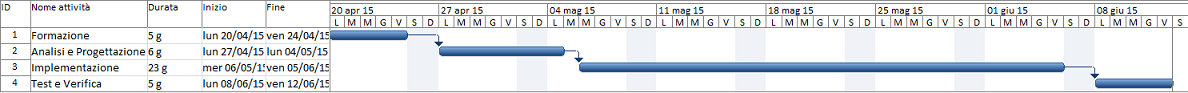
\includegraphics[width=1.1\columnwidth]{gantt_iniziale} 
    \caption{Diagramma Gantt della pianificazione iniziale}
\end{figure}

\subsection{Fase 1: Formazione (40 ore)}
Scopo: formazione sulle problematiche e tecnologie che si incontreranno durante lo stage.
In dettaglio:
\begin{itemize}
	\item angularjs, rest angular, jasmine, istanbul;
	\item ambiente di sviluppo IKS (\gls{ide} per Javascript PhpStorm, Git);
	\item linee guida per lo sviluppo e concetti di programmazione sicura;
	%\item principi di scrittura SOLID
	\item verifica competenze acquisite.
\end{itemize}
Output (oggetto di verifica per il passaggio alla fase successiva):
\begin{itemize}
	\item predisposizione ambiente di sviluppo;
	\item realizzazione di una web application di esempio che utilizzi le tecnologie e gli approcci
indicati.
\end{itemize}

\subsection{Fase 2: Analisi e Progettazione (40 ore)}
Scopo: analisi delle specifiche funzionali, definizione del piano di test e progettazione tecnica
della soluzione da realizzare.\\
In dettaglio:
\begin{itemize}
	\item analisi specifiche funzionali;
	\item progettazione di dettaglio;
	\item documentazione.
\end{itemize}
Output (oggetto di verifica per il passaggio alla fase successiva):
\begin{itemize}
	\item documento di Specifica Tecnica;
	\item User Stories.
\end{itemize}

\subsection{Fase 3: Implementazione (180 ore)}
Scopo: preparazione dell’ambiente di sviluppo e implementazione della soluzione.\\
In dettaglio:
\begin{itemize}
	\item implementazione tecnologica dei requisiti definiti in fase di analisi;
	\item documentazione.
\end{itemize}
Milestone settimanali:
\begin{enumerate}
	\item realizzazione delle funzionalità di dialogo \gls{rest} con il \gls{back-end};
	\item creazione dell'interfaccia del profilo utente singolo;
	\item visione della gerarchia aziendale e dell'organizzazione per progetti dell'organico;
	\item gestione operazioni \gls{crud} sui vari progetti aziendali e sui membri partecipanti.
\end{enumerate}
Output (oggetto di verifica per il passaggio alla fase successiva):
\begin{itemize}
	\item prodotto finale completo in tutte le sue parti;
	\item sorgenti commentati e pubblicati nel repository dei sorgenti aziendale.
\end{itemize}

\subsection{Fase 4: Test e Verifica (40 ore)}
Scopo: Verifica funzionale, dei requisiti e stesura della documentazione.\\
In dettaglio:
\begin{itemize}
	\item analisi dei risultati;
	\item verifica funzionale;
	\item verifica dei requisiti di progetto;
	\item revisione e correzione di eventuali bug;
	\item documentazione;
	\item verifica finale.
\end{itemize}
Output (oggetto di verifica per la conclusione del progetto):
\begin{itemize}
	\item documento finale (conclusioni sull'attività di Stage svolta, con obiettivi raggiunti e
conoscenze acquisite);
	\item eliminazione di bug riscontrati e pubblicazione delle modifiche nel repository dei sorgenti aziendale.
\end{itemize}

%************************************************************************             % Kick-Off
% !TEX encoding = UTF-8
% !TEX TS-program = pdflatex
% !TEX root = ../tesi.tex
% !TEX spellcheck = it-IT

%**************************************************************
\chapter{Analisi dei requisiti}
\label{cap:analisi-requisiti}
%**************************************************************

\intro{Breve introduzione al capitolo}\\

\section{Casi d'uso}

Per lo studio dei casi di utilizzo del prodotto sono stati creati dei diagrammi.
I diagrammi dei casi d'uso (in inglese \emph{Use Case Diagram}) sono diagrammi di tipo \gls{uml} dedicati alla descrizione delle funzioni o servizi offerti da un sistema, così come sono percepiti e utilizzati dagli attori che interagiscono col sistema stesso.\\
Essendo il progetto finalizzato alla creazione di un tool per l'automazione di un processo, le interazioni da parte dell'utilizzatore devono essere ovviamente ridotte allo stretto necessario. Per questo motivo i diagrammi d'uso risultano semplici e in numero ridotto.

\begin{figure}[!h] 
    \centering 
    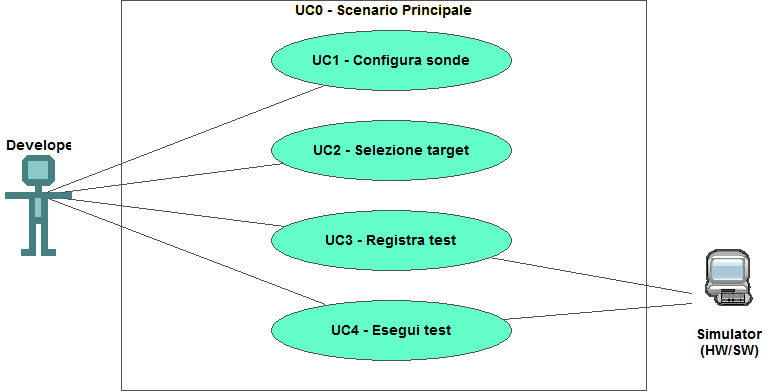
\includegraphics[width=0.9\columnwidth]{usecase/scenario-principale} 
    \caption{Use Case - UC0: Scenario principale}
\end{figure}

\begin{usecase}{0}{Scenario principale}
\usecaseactors{Sviluppatore applicativi}
\usecasepre{Lo sviluppatore è entrato nel plug-in di simulazione all'interno dell'IDE}
\usecasedesc{La finestra di simulazione mette a disposizione i comandi per configurare, registrare o eseguire un test}
\usecasepost{Il sistema è pronto per permettere una nuova interazione}
\label{uc:scenario-principale}
\end{usecase}

\begin{figure}[!h] 
    \centering 
    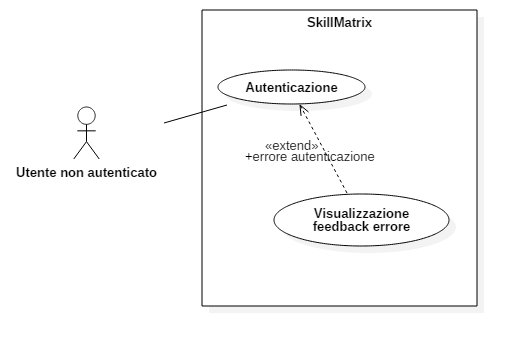
\includegraphics[width=0.9\columnwidth]{usecase/Autenticazione} 
    \caption{Use Case - Login}
\end{figure}

\begin{usecase}{1}{Autenticazione}
\usecaseactors{Utente non autenticato}
\usecasepre{l'utente non ha effettuato il login in SkillMatrix e deve possedere credenziali valide}
\usecasedesc{l'utente fornisce dei dati validi di accesso nella pagina di Login e viene reindirizzato alla pagina di gestione del profilo}
\usecasepost{le credenziali di accesso sono state verificate e l'utente è stato reindirizzato alla DASHBOARD}
\label{uc:autenticazione}
\end{usecase}

\begin{usecase}{2}{Visualizzazione feedback errore}
\usecaseactors{Utente non autenticato}
\usecasepre{l'utente non ha effettuato il login a SkillMatrix}
\usecasedesc{l'utente visualizza un messaggio d'errore nel caso in cui avvenga una delle seguenti situazioni:
\begin{itemize}
	\item le credenziali sono errate;
	\item la comunicazione con il server è fallita.
\end{itemize}}
\usecasepost{viene visualizzato un messaggio d'errore e il contatore che esprime la quantità di volte che l'errore si è manifestato}
\label{uc:errore_login}
\end{usecase}

\begin{figure}[!h] 
    \centering 
    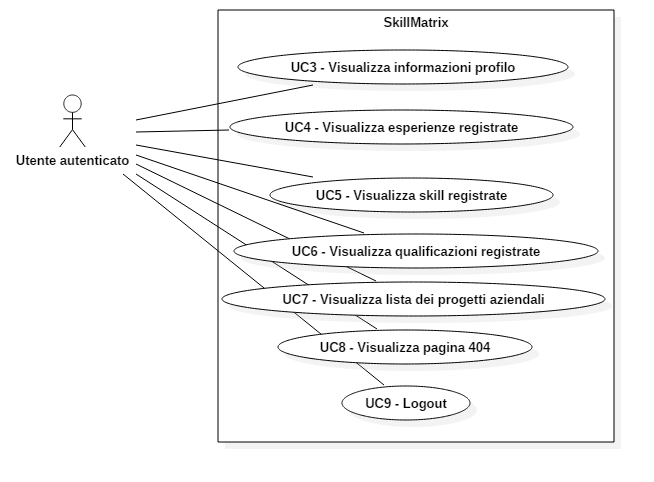
\includegraphics[width=0.9\columnwidth]{usecase/Dashboard} 
    \caption{Use Case - Dashboard}
\end{figure}

\begin{usecase}{3}{Visualizza informazioni profilo}
\usecaseactors{Utente autenticato}
\usecasepre{l'utente deve aver eseguito con successo il login al sistema}
\usecasedesc{l'utente seleziona il menù di visualizzazione delle informazioni del proprio profilo}
\usecasepost{l'utente viene reindirizzato alla pagina di presentazione delle proprie informazioni}
\label{uc:profilo}
\end{usecase}

\begin{usecase}{4}{Visualizza esperienze registrate}
\usecaseactors{Utente autenticato}
\usecasepre{l'utente deve aver eseguito con successo il login al sistema}
\usecasedesc{l'utente seleziona il menù di visualizzazione delle esperienze registrate nel sistema}
\usecasepost{l'utente viene reindirizzato alla pagina di presentazione delle proprie esperienze professionali registrate}
\label{uc:esperienze}
\end{usecase}

\section{Tracciamento dei requisiti}

Da un'attenta analisi dei requisiti e degli use case effettuata sul progetto è stata stilata la tabella che traccia i requisiti in rapporto agli use case.\\
Sono stati individuati diversi tipi di requisiti e si è quindi fatto utilizzo di un codice identificativo per distinguerli.\\
Il codice dei requisiti è così strutturato R(F/Q/V)(N/D/O) dove:
\begin{enumerate}
	  \item[R =] requisito
    \item[F =] funzionale
    \item[Q =] qualitativo
    \item[V =] di vincolo
    \item[N =] obbligatorio (necessario)
    \item[D =] desiderabile
    \item[O =] opzionale
\end{enumerate}
Nelle tabelle \ref{tab:requisiti-funzionali}, \ref{tab:requisiti-qualitativi} e \ref{tab:requisiti-vincolo} sono riassunti i requisiti e il loro tracciamento con gli use case delineati in fase di analisi.

\newpage

\begin{table}%
\caption{Tabella del tracciamento dei requisti funzionali}
\label{tab:requisiti-funzionali}
\begin{tabularx}{\textwidth}{lXl}
\hline\hline
\textbf{Requisito} & \textbf{Descrizione} & \textbf{Use Case}\\
\hline
RFN-1     & (FARLOCCO)L'interfaccia permette di configurare il tipo di sonde del test & UC1 \\
\hline
RFN-1 & L'applicazione deve reagire ad un'errata autenticazione tramite reindirizzamento all'interfaccia di login & UCN \\
\hline
RFN-2 & L'applicazione deve reagire alla scadenza di una sessione tramite reindirizzamento all'interfaccia di login & UCN \\
\hline
RFN-3 & L'applicazione non deve permettere l'accesso anonimo al sistema, tranne che per l'interfaccia di login & UCN \\
\hline
RFN-4 & All'avvio, l'applicazione deve controllare se esiste una sessione attiva & UCN \\
\hline
RFN-5 & In caso di sessione attiva, l'utente deve essere reindirizzato alla Dashboard se la sessione è valida & UCN \\
\hline
RFN-6 & In caso di sessione non attiva o non valida, l'utente deve essere riportato alla schermata di login & UCN \\
\hline
RFN-7 & L'applicazione deve poter consentire ad un utente registrato di effettuare l'autenticazione & UCN \\
\hline
RFN-8 & L'utente autenticato deve poter visionare i propri dati dopo il login nel sistema & UCN \\
\hline
RFN-9 & L'utente autenticato deve poter effettuare il logout dal sistema & UCN \\
\hline
RFN-10 & L'utente deve poter visualizzare i propri titoli di studio e/o abilitazioni professionali una volta effettuato il login & UCN \\
\hline
RFN-11 & L'utente deve poter inserire un nuovo titolo di studio o un'abilitazione professionale nel sistema & UCN \\
\hline
RFN-12 & L'utente deve poter visualizzare le proprie skill una volta effettuato il login & UCN \\
\hline
RFN-12.1 & L'utente deve poter filtrare le skill visualizzate per livello di competenza & UCN \\
\hline
RFN-13 & L'utente deve poter visualizzare i progetti ad esso associati una volta effettuato il login & UCN \\
\hline
RFN-13.1 & L'utente deve poter visualizzare quale progetto necessita di registrazione nel sistema & UCN \\
\hline
RFN-14 & L'utente deve poter visualizzare le informazioni dettagliate di un singolo progetto & UCN \\
\hline
RFN-15 & L'utente deve poter visualizzare le proprie esperienze professionali una volta effettuato il login al sistema & UCN \\
\hline
RFN-16 & L'utente deve poter inserire una nuova esperienza professionale nel sistema & UCN \\
\hline
RFD-1 & Il sistema deve implementare una struttura gerarchica & UCN \\
\hline
RFD-1.1 & L'interfaccia mostrata in base al tipo di ogni utente deve essere adattata al tipo dello stesso & UCN \\
\hline
RFD-1.1.1 & L'amministratore di un progetto deve poter vedere le persone assegnate a quel progetto & UCN \\
\hline
RFD-2 & L'utente deve ricevere un feedback nell'interfaccia ogni volta che avvenga un errore di comunicazione col server & UCN \\
\hline
RFO-1 & Per tutti i dati presentati tramite lista va implementato l'infinite scroll & UCN \\
\hline
RFO-2 & L'utente deve poter visualizzare la quantità di progetti che richiedono registrazione tramite notifica nella dashboard & UCN \\
\hline
\end{tabularx}
\end{table}%

\begin{table}%
\caption{Tabella del tracciamento dei requisiti qualitativi}
\label{tab:requisiti-qualitativi}
\begin{tabularx}{\textwidth}{lXl}
\hline\hline
\textbf{Requisito} & \textbf{Descrizione} & \textbf{Use Case}\\
\hline
RQD-1 & Il codice deve seguire le linee stilistiche aziendali & - \\
\hline
RQD-2 & Deve venire prodotta la documentazione tecnica di dettaglio & - \\
\hline
RQD-3 & La grafica dell'interfaccia deve essere conforme agli standard aziendali & - \\
\hline
RQD-4 & L'utente deve visualizzare una pagina di supporto se naviga verso una pagina non presente & - \\
\hline
\end{tabularx}
\end{table}%

\begin{table}%
\caption{Tabella del tracciamento dei requisiti di vincolo}
\label{tab:requisiti-vincolo}
\begin{tabularx}{\textwidth}{lXl}
\hline\hline
\textbf{Requisito} & \textbf{Descrizione} & \textbf{Use Case}\\
\hline
RVN-1 & Il framework di sviluppo per l'applicazione frontend dev'essere AngularJS & - \\
\hline
RVN-2 & La libreria css da utilizzare dev'essere Bootstrap & - \\
\hline
RVN-3 & Il framework di testing da utilizzare deve essere Jasmine & - \\
\hline
RVN-4 & L'approccio di sviluppo deve essere Test Driven & - \\
\hline
RVN-5 & Devono essere realizzate una o più componenti che simulino il backend in assenza di un server funzionante & - \\
\hline
RVN-6 & Le API definite devono rispettare il paradigma REST/HATEOAS & - \\
\hline
RVN-6.1 & L'interfaccia deve poter manipolare correttamente gli header HTTP & - \\
\hline
RVN-7 & L'assegnamento dei ticket deve essere eseguito tramite il sistema kanban (JIRA) & - \\
\hline
RVN-8 & Il repository da utilizzare deve essere la configurazione aziendale di Atlassian STASH & - \\
\hline
RVN-9 & Lo schema dei dati associati ad un utente deve essere preso da schema.org & - \\
\hline
RVO-1 & I dati tabellari devono essere richiesti al server in maniera paginata & - \\
\hline
\end{tabularx}
\end{table}%             % Concept Preview
% !TEX encoding = UTF-8
% !TEX TS-program = pdflatex
% !TEX root = ../tesi.tex
% !TEX spellcheck = it-IT

%**************************************************************
\chapter{Progettazione e codifica}
\label{cap:progettazione-codifica}
%**************************************************************

\intro{Breve introduzione al capitolo}\\

%**************************************************************

\section{Angular MVC}
AngularJS è stato il framework maggiormente utilizzato in questo stage e mi ha consentito di implementare l'intero progetto agilmente.\\
Alla base del framework, è collocato il design pattern \gls{mvc}, leggermente modificato per adattarsi alle funzionalità di AngularJS. Il design pattern che ne risulta è qualcosa di più flessibile del classico \gls{mvc}, consentendo agli sviluppatori una maggior libertà di utilizzo.\\
Ovviamente ci sono delle direttive e delle best practice consigliate, soprattutto se si intende creare un \gls{frontend} davvero \gls{rest}-ful.

\subsection{Two-way Data Binding}
Una funzionalità importante che AngularJS espone è il cosiddetto \emph{Two Way Data Binding}. Si parla di \emph{legame doppio tra dati} quando una variabile del modello è legata ad un elemento che può cambiare ed al contempo mostrare il contenuto della variabile stessa. In una vista di AngularJS, ogniqualvolta un elemento che applica il \emph{Two Way Data Binding} viene modificato, il corrispondente campo nel modello viene notificato e aggiornato correttamente.\\
In AngularJS, si usa la direttiva \textbf{ng-model} per legare una variabile del modello ad un elemento \gls{html} che può sia mostrare il suo valore, che modificarlo.

\begin{figure}[H] 
    \centering 
    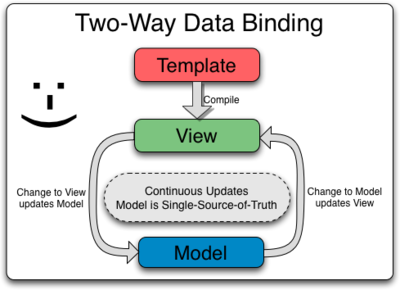
\includegraphics[width=0.8\columnwidth]{two_way_data_binding} 
    \caption{Doppio legame tra vista e modello di AngularJS}
\end{figure}




%**************************************************************

\section{Tecnologie e strumenti}
\label{sec:tecnologie-strumenti}

Di seguito viene data una panoramica delle tecnologie e strumenti utilizzati.

\subsection*{Tecnologia 1}
Descrizione Tecnologia 1.

\subsection*{Tecnologia 2}
Descrizione Tecnologia 2

%**************************************************************
\section{Ciclo di vita del software}
\label{sec:ciclo-vita-software}

%**************************************************************
\section{Progettazione}
\label{sec:progettazione}

\subsubsection{Namespace 1} %**************************
Descrizione namespace 1.

\begin{namespacedesc}
    \classdesc{Classe 1}{Descrizione classe 1}
    \classdesc{Classe 2}{Descrizione classe 2}
\end{namespacedesc}


%**************************************************************
\section{Design Pattern utilizzati}

%**************************************************************
\section{Codifica}
             % Product Prototype
% !TEX encoding = UTF-8
% !TEX TS-program = pdflatex
% !TEX root = ../tesi.tex
% !TEX spellcheck = it-IT

%**************************************************************
\chapter{Verifica e validazione}
\label{cap:verifica-validazione}
%**************************************************************             % Product Design Freeze e SOP
% !TEX encoding = UTF-8
% !TEX TS-program = pdflatex
% !TEX root = ../tesi.tex
% !TEX spellcheck = it-IT

%**************************************************************
\chapter{Conclusioni}
\label{cap:conclusioni}
%**************************************************************

%**************************************************************
\section{Bilancio finale}

%**************************************************************
\section{Problematiche incontrate}
L'applicazione di un modello di sviluppo \emph{Agile} è stata relativamente difficoltosa, a primo impatto. Questo modello, a mio avviso, si applica più efficacemente a sviluppatori con solida esperienza, data la sua versatilità e flessibilità di utilizzo. Infatti, se si applica la metodologia \emph{Agile} senza delle procedure adeguate, il risultato può essere imprevedibile.\\
Sebbene all'interno dell'azienda ci fossero delle procedure ben consolidate per l'applicazione di questo modello, la sua attuazione da parte mia non è stata immediata. Ciò è stato anche causato dall'assenza di esperienza da parte mia delle tecnologie aziendali per la gestione dello sviluppo software, per colmare la quale è stata impiegata la prima settimana di Stage.\\
La settimana iniziale di formazione ha contribuito ampiamente a colmare le mie lacune teoriche e pratiche sull'attuazione di una metodologia \emph{Agile} e sulla sua implementazione a livello di strumenti aziendali.\\
Ho riscontrato la stessa mancanza di conoscenze per quanto riguarda gli strumenti di automazione e di testing che ho utilizzato in questo Stage. Questo problema è stato facilmente risolvibile, in quanto la documentazione presente online dei framework che ho utilizzato è ampiamente esaustiva; inoltre la facilità di interfacciamento tra le varie componenti dello stack tecnologico che ho utilizzato, ha permesso una ancora maggiore efficienza nell'apprendimento e nell'applicazione di queste tecnologie.\\
Per ultima, forse la realtà che è stata più distante dalla mia consuetudine di studente, la metodologia \emph{test driven} si è rivelata tanto efficace quanto difficile da applicare. Il metodo di sviluppo che sta alla base del \emph{test driven developement} è stato molto lontano da quello che ho applicato nei progetti della mia carriera universitaria.

%**************************************************************
\section{Conoscenze acquisite}
L'acquisizione delle conoscenze necessarie ad applicare la metodologia \emph{Agile} con criterio e organizzazione è stata per me un obiettivo fondamentale per la buona riuscita dello Stage e per la mia carriera futura. Sicuramente l'aggiunta dei framework che implementano questa tecnologia che ho imparato a conoscere durante lo Stage ampliano molto il mio bagaglio culturale di sviluppatore.\\
Ritengo che la metodologia di sviluppo \emph{Agile}, se applicata con criterio, sia molto efficace e durante il corso di questo Stage ho imparato a mettere in pratica i suoi principi, grazie anche all'aiuto del mio Responsabile aziendale Marco Albarelli.\\
Un'altra metodologia che sono stato molto soddisfatto di aver applicato è il \emph{test driven developement}. Sebbene il primo impatto spinga a vedere lo sviluppo \emph{test driven} come molto oneroso in termine di tempo e, forse, ripetitività, a lungo andare gli effetti di un investimento iniziale sono molto positivi. Questa metodologia permette di risparmiare molto lavoro postumo e aumenta la manutenibilità del codice, garantendo la qualità del codice stesso ancora prima della sua stesura. Inoltre, quando si ha a che fare con linguaggi di programmazione molto liberi come \emph{JavaScript}, l'apporto di test alla scrittura di codice è pressoché obbligatorio, se davvero si vogliono scrivere applicazioni stabili e manutenibili.\\
Ultimo ma non meno importante, ho potuto esprimere al meglio il mio interesse verso il \emph{framework} AngularJS. Questo \emph{framework}, oltre ad avere delle funzionalità molto utili per lo sviluppo di applicazioni \gls{front-end}, garantisce una compatibilità molto alta con altri strumenti utili per lo sviluppo di applicazioni \emph{client-side}, come gli strumenti di testing e automazione.\\
La scrittura di applicazioni web con AngularJS e Bootstrap risulta molto intuitiva e veloce, soprattutto se supportatat da strumenti come Grunt e Karma, che ho imparato ad utilizzare approfonditamente durante questo Stage. 

%**************************************************************
\section{Valutazione personale}
La mia valutazione personale sull'attività di Stage che ho svolto è estremamente positiva. Il confronto con una realtà lavorativa mi ha portato all'acquisizione di esperienze più profonde e concrete rispetto ad un progetto didattico.\\
Il personale di IKS è stato sempre molto disponibile a chiarire i miei dubbi, invitandomi a partecipare attivamente ed a riflettere sulle soluzioni da adottare, così da farmi crescere ulteriormente sia come sviluppatore che come persona; ringrazio davvero molto l'azienda e l'università per avermi concesso questa opportunità.\\
Infine penso che le tecnologie che ho applicato durante lo Stage mi saranno utili nel futuro prossimo, sia che le vada ad applicare direttamente, sia che vada ad adottare un diverso \emph{stack} tecnologico. In ogni caso, ho aumentato la mia sicurezza  ed efficienza nell'applicazione di queste conoscenze, e penso che ciò sia molto utile.

             % Conclusioni
\appendix                               
% !TEX encoding = UTF-8
% !TEX TS-program = pdflatex
% !TEX root = ../tesi.tex
% !TEX spellcheck = it-IT

%**************************************************************
\chapter{Appendice A}
%**************************************************************

\epigraph{Citazione}{Autore della citazione}



             % Appendice A

%**************************************************************
% Materiale finale
%**************************************************************
\backmatter
\printglossaries
% !TEX encoding = UTF-8
% !TEX TS-program = pdflatex
% !TEX root = ../tesi.tex
% !TEX spellcheck = it-IT

%**************************************************************
% Bibliografia
%**************************************************************

\cleardoublepage
\chapter{Bibliografia}

\nocite{*}
%\printbibliography

\bibbycategory % equivale a dare un \printbibliography per ogni categoria


\end{document}